
\subsection{The Filesystem}

% TODO namespace, data objects / inodes

We model a filesystem using a function $\FS$ with a set of nodes (filesystem paths) $\setn$ as its domain,
and a set of possible contents or values, $\setv$, as its codomain:
\[ \FS : \setn \rightarrow \setv \] 
In our model, $\setn$ 
serves as a namespace or ``skeleton'' for the filesystem, and it
contains all possible nodes, including the ones where there is no file or directory.
To model empty nodes, $\setv$ 
contains a special element ($\empt$) which is the value of $\FS$ at these nodes.
We consider the contents of files, as well as any meta-information of files
and directories (e.g. permissions and other flags) part of the values in $\setv$.


The nodes form a disjoint union of rooted directed trees.
\begin{mydef}
The function $\parent(n)$ returns the parent node of $n$, or
returns $\topnode$ if $n$ is the root of a tree.
\end{mydef}

Every filesystem has a so-called \textbf{tree property}, which means that
if the filesystem is not empty at a node, and the node has a parent,
then there must be a directory at the parent node.

To model this, in $\setv$ we distinguish between 
file contents ($\setf$) and directory contents ($\setd$), that is,
if $\setb = \{\empt\}$ then:
\[ \setv = \setb \cup \setf \cup \setd \]
The tree property can then be defined as
\begin{align*}
\forall n\in\setn: &\FS(n) \neq \empt \\ % TODO alignment problem
&\quad\wedge \parent(n) \neq \topnode \\
&\Rightarrow \FS(\parent(n)) \in \setd 
\end{align*}
This means that as we move down from the root of a tree of nodes,
the types of values we encounter in the filesystem can only change according to the
transition diagram in \cref{fig_transition}.

\begin{figure}[htb]
\begin{center}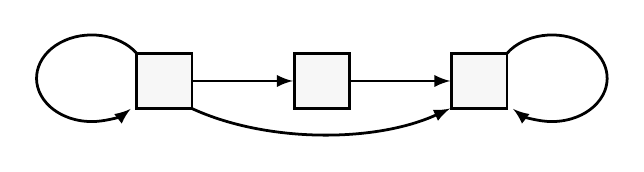
\begin{tikzpicture}
 [line width=1pt, bend angle=45,
 sq/.style={rectangle,inner sep=3pt, minimum size=7mm,
fill=black!3,draw=black}]
\node[sq] (dnode) at (0,0) {$\cchard$};
\node[sq] (fnode) at (2,0) {$\ccharf$};
\node[sq] (bnode) at (4,0) {$\ccharb$};
\draw[-latex] (dnode) -- (fnode);
\draw[-latex] (fnode) -- (bnode);
\draw[-latex] (-0.35,  0.35) arc(35:315:0.7cm and 0.55cm);
\draw[-latex] ( 4.35,  0.35) arc(145:-135:0.7cm and 0.55cm);
\draw[-latex] ( 0.35, -0.35) arc(230:310:2.55cm and 1.4cm);
\end{tikzpicture}\end{center}
\caption{Transitions between types of values in a filesystem}\label{fig_transition}
\end{figure}

In this paper, $n$, $m$ and $o$ denote nodes in $\setn$.
We use $\valf$ for an arbitrary element in $\setf$, 
and $\vald$ for an arbitrary element in $\setd$,
and by $\valvx$ we mean a value of type $X$ in $\setvx{X}$.



Another simplification we will assume in this paper is regarding directories.
As Bill Zissimopoulos pointed out (\cite{BZ}), we often do not want to consider metadata stored in
directories during synchronization. In other words, the contents of directories are all equal,
which can be modelled by assuming that $|\setd|=1$.
% This also creates a convenient symmetry where there is only a single value
% for each type that can be repeated as we move from a path to its child ($D$ and $\empt$).
